\documentclass{article}
\usepackage[top=3cm, bottom=3cm, outer=3cm, inner=3cm]{geometry}
\usepackage{multicol}
\usepackage{graphicx}
\usepackage{url}
%\usepackage{cite}
\usepackage{hyperref}
\usepackage{array}
%\usepackage{multicol}
\newcolumntype{x}[1]{>{\centering\arraybackslash\hspace{0pt}}p{#1}}
\usepackage{natbib}
\usepackage{pdfpages}
\usepackage{multirow}
\usepackage[normalem]{ulem}
\useunder{\uline}{\ul}{}
\usepackage{svg}
\usepackage{xcolor}
\usepackage{listings}
\lstdefinestyle{ascii-tree}{
    literate={├}{|}1 {─}{--}1 {└}{+}1 
  }
\lstset{basicstyle=\ttfamily,
  showstringspaces=false,
  commentstyle=\color{red},
  keywordstyle=\color{blue}
}
%\usepackage{booktabs}
\usepackage{caption}
\usepackage{subcaption}
\usepackage{float}
\usepackage{array}

\newcolumntype{M}[1]{>{\centering\arraybackslash}m{#1}}
\newcolumntype{N}{@{}m{0pt}@{}}


%%%%%%%%%%%%%%%%%%%%%%%%%%%%%%%%%%%%%%%%%%%%%%%%%%%%%%%%%%%%%%%%%%%%%%%%%%%%
%%%%%%%%%%%%%%%%%%%%%%%%%%%%%%%%%%%%%%%%%%%%%%%%%%%%%%%%%%%%%%%%%%%%%%%%%%%%
\newcommand{\itemEmail}{lflorezb@unsa.edu.pe}
\newcommand{\itemStudent}{Grupo 08}
\newcommand{\itemB}{Florez Bailon Luis Fernando}
\newcommand{\itemC}{Champi Sanchez Manuel Mario}
\newcommand{\itemDocente}{Mg. Edith Giovanna Cano Mamani}
\newcommand{\itemCourse}{Laboratorio EDA}
\newcommand{\itemCourseCode}{1702122}
\newcommand{\itemSemester}{III}
\newcommand{\itemUniversity}{Universidad Nacional de San Agustín de Arequipa}
\newcommand{\itemFaculty}{Facultad de Ingeniería de Producción y Servicios}
\newcommand{\itemDepartment}{Departamento Académico de Ingeniería de Sistemas e Informática}
\newcommand{\itemSchool}{Escuela Profesional de Ingeniería de Sistemas}
\newcommand{\itemAcademic}{2023 - A}
\newcommand{\itemInput}{Del 19 Julio 2023}
\newcommand{\itemOutput}{Al 23 Julio 2023}
\newcommand{\itemPracticeNumber}{06}
\newcommand{\itemTheme}{Tries}
%%%%%%%%%%%%%%%%%%%%%%%%%%%%%%%%%%%%%%%%%%%%%%%%%%%%%%%%%%%%%%%%%%%%%%%%%%%%
%%%%%%%%%%%%%%%%%%%%%%%%%%%%%%%%%%%%%%%%%%%%%%%%%%%%%%%%%%%%%%%%%%%%%%%%%%%%

\usepackage[english,spanish]{babel}
\usepackage[utf8]{inputenc}
\AtBeginDocument{\selectlanguage{spanish}}
\renewcommand{\figurename}{Figura}
\renewcommand{\refname}{Referencias}
\renewcommand{\tablename}{Tabla} %esto no funciona cuando se usa babel
\AtBeginDocument{%
	\renewcommand\tablename{Tabla}
}

\usepackage{fancyhdr}
\pagestyle{fancy}
\fancyhf{}
\setlength{\headheight}{30pt}
\renewcommand{\headrulewidth}{1pt}
\renewcommand{\footrulewidth}{1pt}
\fancyhead[L]{\raisebox{-0.2\height}{
\includegraphics[width=3cm]{img/logo_episunsa.png}}}
\fancyhead[C]{\fontsize{7}{7}\selectfont	\itemUniversity \\ \itemFaculty \\ \itemDepartment \\ \itemSchool \\ \textbf{\itemCourse}}
\fancyhead[R]{\raisebox{-0.2\height}{
\includegraphics[width=1.2cm]{img/logo_abet}}}
\fancyfoot[L]{\itemStudent}
\fancyfoot[C]{\itemCourse}
\fancyfoot[R]{Página \thepage}

% para el codigo fuente
\usepackage{listings}
\usepackage{color, colortbl}
\definecolor{dkgreen}{rgb}{0,0.6,0}
\definecolor{gray}{rgb}{0.5,0.5,0.5}
\definecolor{mauve}{rgb}{0.58,0,0.82}
\definecolor{codebackground}{rgb}{0.95, 0.95, 0.92}
\definecolor{tablebackground}{rgb}{0.8, 0, 0}

\lstset{frame=tb,
	language=bash,
	aboveskip=3mm,
	belowskip=3mm,
	showstringspaces=false,
	columns=flexible,
	basicstyle={\small\ttfamily},
	numbers=none,
	numberstyle=\tiny\color{gray},
	keywordstyle=\color{blue},
	commentstyle=\color{dkgreen},
	stringstyle=\color{mauve},
	breaklines=true,
	breakatwhitespace=true,
	tabsize=3,
	backgroundcolor= \color{codebackground},
}

\begin{document}

	\vspace*{10px}
	\begin{center}	
		\fontsize{17}{17} \textbf{ Informe de Laboratorio \itemPracticeNumber}
	\end{center}
	\centerline{\textbf{\Large Tema: \itemTheme}}
	%\vspace*{0.5cm}
 
	\begin{flushright}
		\begin{tabular}{|M{2.5cm}|N|}
			\hline 
			\rowcolor{tablebackground}
			\color{white} \textbf{Nota}  \\
			\hline 
			     \\[30pt]
			\hline 			
		\end{tabular}
	\end{flushright}	

	\begin{table}[H]
		\begin{tabular}{|x{5cm}|x{4.8cm}|x{4.8cm}|}
			\hline 
			\rowcolor{tablebackground}
			\color{white} \textbf{Estudiantes} & \color{white}\textbf{Docente}  & \color{white}\textbf{Asignatura}   \\
			\hline 
			{\itemB \par \itemA \par \itemC \par \itemD} & \itemDocente & {\itemCourse \par Semestre: \itemSemester \par Código: \itemCourseCode}     \\
			\hline 			
		\end{tabular}
	\end{table}		
	
	\begin{table}[H]
		\begin{tabular}{|x{4.7cm}|x{4.8cm}|x{4.8cm}|}
			\hline 
			\rowcolor{tablebackground}
			\color{white}\textbf{Laboratorio} & \color{white}\textbf{Tema}  & \color{white}\textbf{Duración}   \\
			\hline 
			\itemPracticeNumber & \itemTheme & 04 horas   \\
			\hline 
		\end{tabular}
	\end{table}
	
	\begin{table}[H]
		\begin{tabular}{|x{4.7cm}|x{4.8cm}|x{4.8cm}|}
			\hline 
			\rowcolor{tablebackground}
			\color{white}\textbf{Semestre académico} & \color{white}\textbf{Fecha de inicio}  & \color{white}\textbf{Fecha de entrega}   \\
			\hline 
			\itemAcademic & \itemInput &  \itemOutput  \\
			\hline 
		\end{tabular}
	\end{table}
	
	
	
		
	
	
	\section{URL de Repositorio Github}
	\begin{itemize}
		\item URL del Repositorio GitHub para clonar o recuperar.
		\item \url{https://github.com/ManuelChampi/Eda_Lab_D23A}
		\item URL para el laboratorio 06 en el Repositorio GitHub.
		\item \url{https://github.com/ManuelChampi/Eda_Lab_D23A/tree/main/Eda_Lab_06}
	\end{itemize}
	\clearpage
	\section{Actividades con el repositorio GitHub}
	
	\subsection{Resolución de ejercicio}
          \subsubsection{Clase TrieGUI}
          \begin{itemize}
              \item Se crea la interfaz gráfica de usuario.
          \end{itemize}
          \begin{figure}[H]
              \centering
              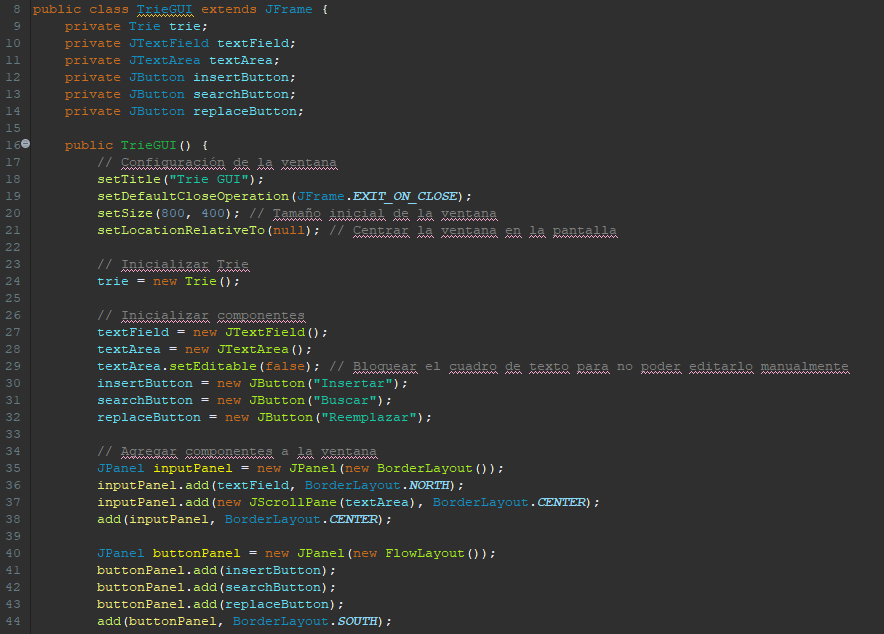
\includegraphics[scale=0.79]{img/img1.png}
              \caption{Constructor TriGUI}
              \label{fig:enter-label}
          \end{figure}
          \clearpage
          \begin{itemize}
              \item Creamos los respectivos listeners para los botones insertar, buscar y reemplazar.
          \end{itemize}
          \begin{figure}[H]
              \centering
              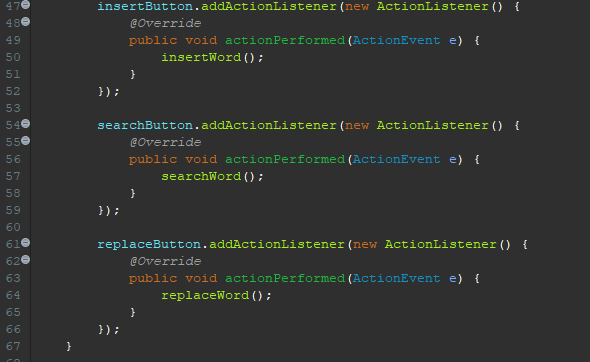
\includegraphics{img/img2.png}
              \caption{Listeners para los botones}
              \label{fig:enter-label}
          \end{figure}
          \begin{itemize}
              \item El método insertWord nos permitirá ingresar el texto que el usuario desee.
          \end{itemize}
          \begin{figure}[H]
              \centering
              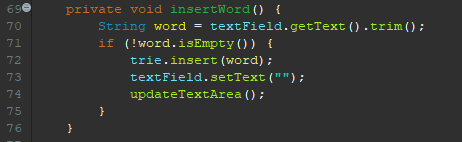
\includegraphics{img/img3.png}
              \caption{Metodo insertWord}
              \label{fig:enter-label}
          \end{figure}
          \clearpage
          \begin{itemize}
              \item El método searchWord nos permite buscar una palabra específica que sea ingresada por el usuario. Si la palabra no está vacía, busca la cantidad de apariciones de esa palabra en el texto utilizando indexOf y muestra un mensaje con el resultado.
          \end{itemize}
          \begin{figure}[H]
              \centering
              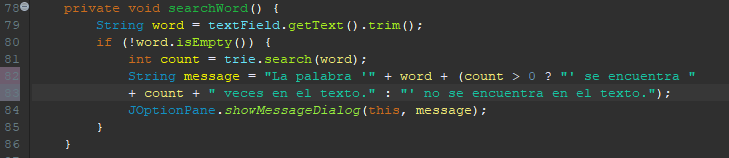
\includegraphics[scale=0.8]{img/img4.png}
              \caption{Metodo searchWord}
              \label{fig:enter-label}
          \end{figure}
          \begin{itemize}
              \item El método replaceWord nos pide ingresar una palabra, luego el programa buscará todas las palabras iguales en el texto y las reemplaza por la palabra que indiquemos. Luego actualiza el área de texto para mostrar el texto modificado.
          \end{itemize}
          \begin{figure}[H]
              \centering
              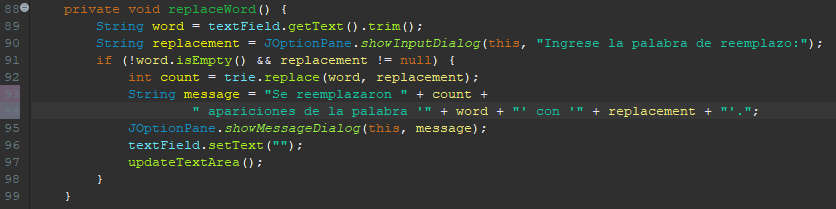
\includegraphics[scale=0.8]{img/img5.png}
              \caption{Metodo replaceWord}
              \label{fig:enter-label}
          \end{figure}
          \begin{itemize}
              \item Método para actualizar el área de texto con el texto almacenado en la Trie. Formatea el texto almacenado en la Trie para ajustarlo al ancho del área de texto, realizando un salto de línea cuando el texto supere el ancho de la ventana.
          \end{itemize}
          \begin{figure}[H]
              \centering
              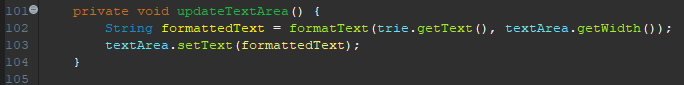
\includegraphics{img/img6.png}
              \caption{Metodo updateTextArea}
              \label{fig:enter-label}
          \end{figure}
          \clearpage
          \begin{itemize}
              \item Método para formatear el texto para ajustarlo al ancho del área de texto.
          \end{itemize}
          \begin{figure}[H]
              \centering
              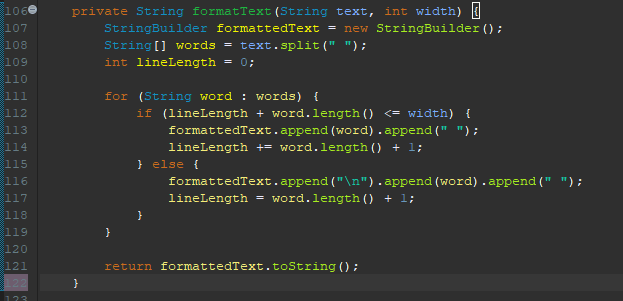
\includegraphics{img/img7.png}
              \caption{Metodo formatText}
              \label{fig:enter-label}
          \end{figure}
          \begin{itemize}
              \item Se crea el main para poder correr el programa.
          \end{itemize}
	 \begin{figure}[H]
	     \centering
	     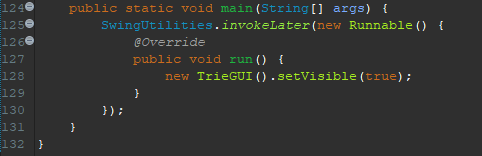
\includegraphics{img/img8.png}
	     \caption{Main}
	     \label{fig:enter-label}
	 \end{figure}
  \clearpage
  \subsubsection{Clase Trie}
   \begin{itemize}
       \item Clase que representa la estructura de datos Trie. Tiene un nodo raíz y un StringBuilder para almacenar el texto ingresado. Permite insertar palabras en la Trie, realizar búsqueda de palabras y reemplazar palabras en el texto..
   \end{itemize}
   \begin{figure}[H]
       \centering
       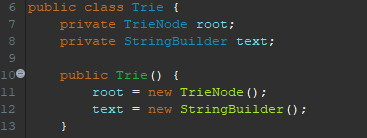
\includegraphics{img/img9.png}
       \caption{constructor Trie}
       \label{fig:enter-label}
   \end{figure}
   \begin{itemize}
        \item “insert(String word)” es un método para insertar una palabra en la Trie. Recibe una palabra como parámetro y la inserta en la Trie. Comienza en el nodo raíz y recorre cada carácter de la palabra. Para cada carácter, verifica si ya existe un nodo hijo con ese carácter en el nodo actual. Si no existe, crea un nuevo nodo hijo con ese carácter. Luego, avanza al nodo hijo correspondiente. Una vez que ha recorrido todos los caracteres de la palabra, marca el último nodo como el final de una palabra (isEndOfWord se establece en true) y agrega la palabra al StringBuilder text, seguida de un espacio en blanco.
   \end{itemize}
   \begin{figure}[H]
       \centering
       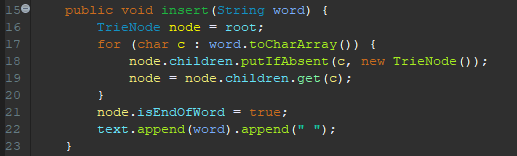
\includegraphics{img/img10.png}
       \caption{Metodo insert}
       \label{fig:enter-label}
   \end{figure}
   \clearpage
   \begin{itemize}
        \item “search(String word)” es un método para buscar una palabra en la Trie. Recibe una palabra como parámetro y busca la cantidad de apariciones de esa palabra en el texto almacenado en la Trie. Utiliza el método indexOf del StringBuilder text para buscar la palabra en el texto. Inicialmente, count se establece en 0. Mientras encuentre la palabra en el texto (indexOf devuelve un índice válido), incrementa count y busca la siguiente aparición de la palabra a partir del índice siguiente. El método devuelve la cantidad de apariciones encontradas.
   \end{itemize}
   \begin{figure}[H]
       \centering
       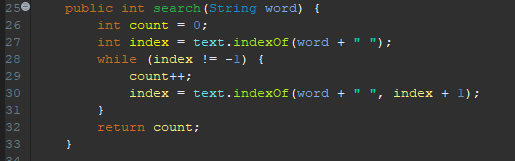
\includegraphics{img/img11.png}
       \caption{Metodo search}
       \label{fig:enter-label}
   \end{figure}
   \begin{itemize}
    \item “replace(String word, String replacement)” es un método para reemplazar una palabra en la Trie. Recibe dos parámetros: word es la palabra que se va a reemplazar y replacement es la palabra de reemplazo. Busca la primera aparición de word en el texto utilizando indexOf. Mientras encuentre word en el texto (indexOf devuelve un índice válido), reemplaza la palabra con replacement utilizando el método replace del StringBuilder. Incrementa count para mantener un registro de cuántos reemplazos se han realizado. Luego, busca la siguiente aparición de word a partir del índice siguiente al reemplazo realizado. El método devuelve la cantidad de reemplazos realizados.
   \end{itemize}
   \begin{figure}[H]
       \centering
       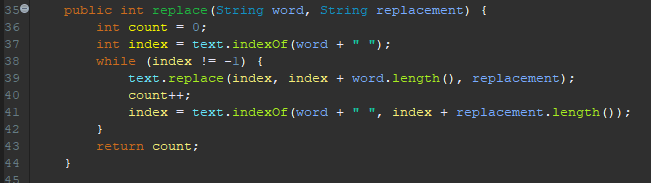
\includegraphics{img/img 12.png}
       \caption{Metodo replace}
       \label{fig:enter-label}
   \end{figure}
   \clearpage
   \begin{itemize}
       \item “getText()” es el método para obtener el texto almacenado en la Trie. Devuelve el texto almacenado en el StringBuilder text como una cadena de caracteres.
   \end{itemize}
   \begin{figure}[H]
       \centering
       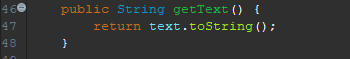
\includegraphics{img/img13.png}
       \caption{Metodo getText}
       \label{fig:enter-label}
   \end{figure}
   \begin{itemize}
       \item “TrieNode” es una clase interna que representa un nodo de la Trie. Tiene dos atributos: children, que es un mapa que mantiene las relaciones entre los caracteres y los nodos hijos, y isEndOfWord, un indicador que determina si este nodo es el final de una palabra. El constructor TrieNode() inicializa el mapa children como un nuevo HashMap y isEndOfWord como false.
   \end{itemize}
   \begin{figure}[H]
       \centering
       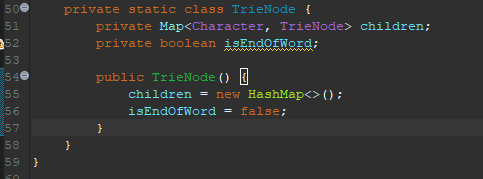
\includegraphics{img/img14.png}
       \caption{Clase TrieNode}
       \label{fig:enter-label}
   \end{figure}
   
   \clearpage
\subsection{Pruebas}
 \begin{itemize}
        \item \textbf{Insertar}
 \end{itemize}
 \begin{figure}[H]
       \centering
       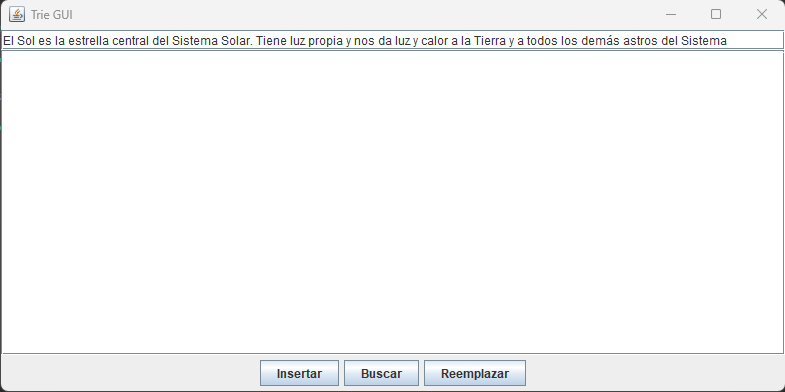
\includegraphics[scale=0.79]{img/img15.png}
       \caption{Ingresar texto}
       \label{fig:enter-label}
 \end{figure}
 \begin{figure}[H]
       \centering
       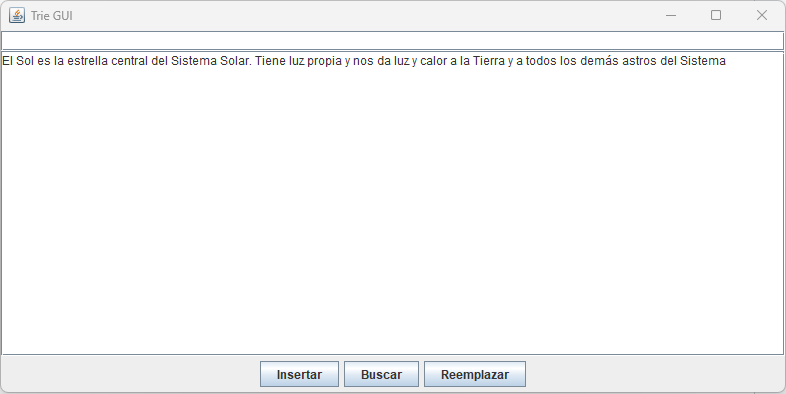
\includegraphics[scale=0.79]{img/img16.png}
       \caption{Mostrar texto}
       \label{fig:enter-label}
 \end{figure}
\clearpage
\begin{itemize}
    \item \textbf{Buscar}
\end{itemize}
\begin{figure}[H]
       \centering
       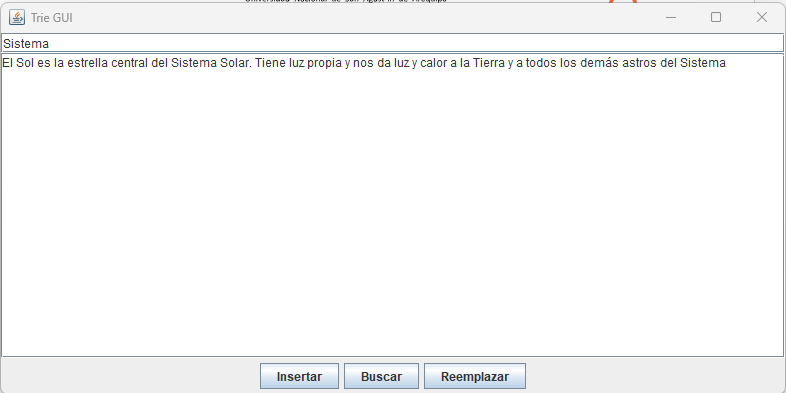
\includegraphics[scale=0.79]{img/img17.png}
       \caption{Ingresar palabra}
       \label{fig:enter-label}
 \end{figure}
 \begin{figure}[H]
       \centering
       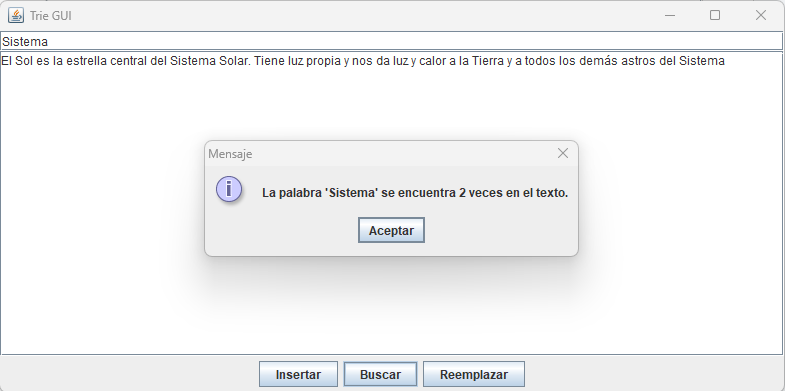
\includegraphics[scale=0.79]{img/img18.png}
       \caption{Mensaje de busqueda}
       \label{fig:enter-label}
 \end{figure}
 \clearpage
\begin{itemize}
    \item \textbf{Reemplazar}
\end{itemize}
 \begin{figure}[H]
       \centering
       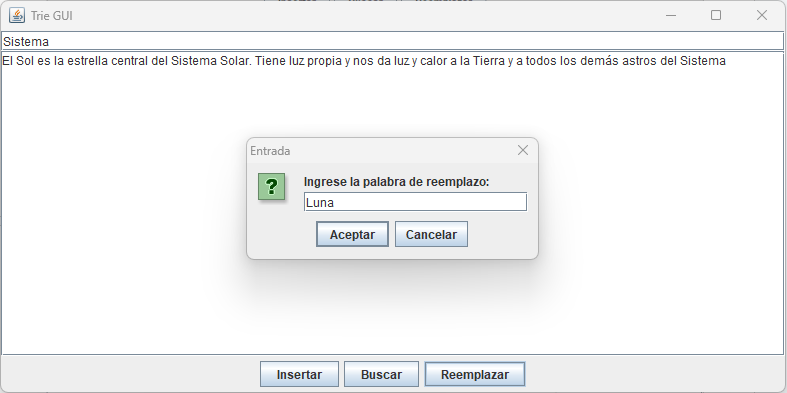
\includegraphics[scale=0.79]{img/img19.png}
       \caption{MPalabra a reemplazar}
       \label{fig:enter-label}
 \end{figure}
  \begin{figure}[H]
       \centering
       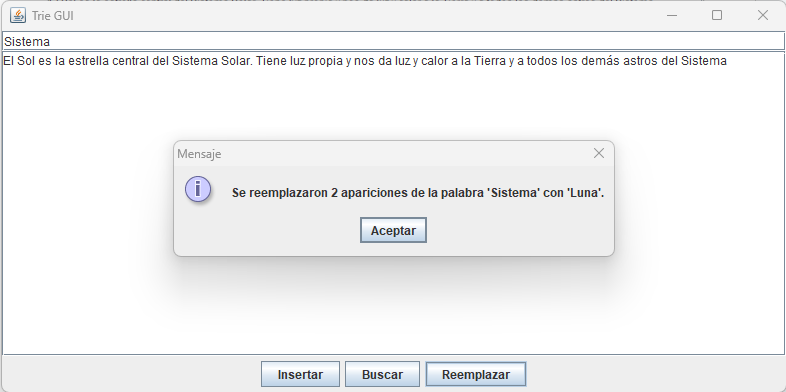
\includegraphics[scale=0.79]{img/img20.png}
       \caption{Mensaje de reemplazo}
       \label{fig:enter-label}
 \end{figure}
 \clearpage
   \begin{figure}[H]
       \centering
       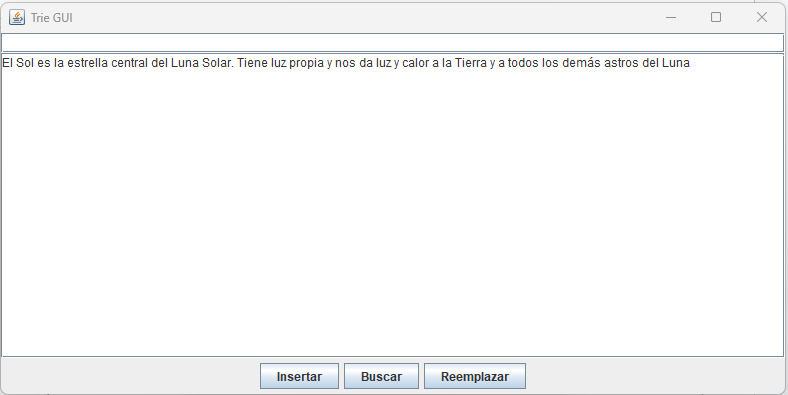
\includegraphics[scale=0.79]{img/img21.png}
       \caption{Resultado de reemplazo}
       \label{fig:enter-label}
 \end{figure}
\clearpage


\subsection{Resolución de cuestionario}
 \begin{itemize}
     \item \textbf{Explique. ¿Cómo se utiliza esta estructura de datos para almacenar prefijos?.}
 \end{itemize}
 \newline
 La estructura de datos Trie es especialmente útil para almacenar y buscar palabras o cadenas de caracteres de manera eficiente. Se utiliza comúnmente en tareas que involucran búsqueda rápida de palabras o prefijos, como autocompletar en motores de búsqueda, correctores ortográficos y sistemas de búsqueda de palabras clave.
\begin{itemize}
     \item \textbf{¿Cómo realizo la funcionalidad de reemplazar texto?}
 \end{itemize}
 \newline
Recibe dos parámetros: word es la palabra que se va a reemplazar y replacement es la palabra de reemplazo. Busca la primera aparición de word en el texto utilizando indexOf. Mientras encuentre word en el texto (indexOf devuelve un índice válido), reemplaza la palabra con replacement utilizando el método replace del StringBuilder. Incrementa count para mantener un registro de cuántos reemplazos se han realizado. Luego, busca la siguiente aparición de word a partir del índice siguiente al reemplazo realizado. El método devuelve la cantidad de reemplazos realizados.	
\end{document}
